\documentclass[a4paper,twoside]{article}
\usepackage[T1]{fontenc}
\usepackage[bahasa]{babel}
\usepackage{graphicx}
\usepackage{graphics}
\usepackage{float}
\usepackage[cm]{fullpage}
\pagestyle{myheadings}
\usepackage{etoolbox}
\usepackage{setspace} 
\usepackage{lipsum} 
\setlength{\headsep}{30pt}
\usepackage[inner=2cm,outer=2.5cm,top=2.5cm,bottom=2cm]{geometry} %margin
% \pagestyle{empty}

\makeatletter
\renewcommand{\@maketitle} {\begin{center} {\LARGE \textbf{ \textsc{\@title}} \par} \bigskip {\large \textbf{\textsc{\@author}} }\end{center} }
\renewcommand{\thispagestyle}[1]{}
\markright{\textbf{\textsc{Laporan Perkembangan Pengerjaan Skripsi\textemdash Sem. Genap 2022/2023}}}

\onehalfspacing
 
\begin{document}

\title{\@judultopik}
\author{\nama \textendash \@npm} 

%ISILAH DATA BERIKUT INI:
\newcommand{\nama}{Bosnich Timothy Bonsaleng}
\newcommand{\@npm}{2017730086}
\newcommand{\tanggal}{13/06/2023} %Tanggal pembuatan dokumen
\newcommand{\@judultopik}{Pemvisualisasi Hasil Penelitian Area Hijau
	Kelurahan} % Judul/topik anda
\newcommand{\kodetopik}{PAN5491}
\newcommand{\jumpemb}{1} % Jumlah pembimbing, 1 atau 2
\newcommand{\pembA}{Pascal~Alfadian,~Nugroho,~M.Comp.}
\newcommand{\pembB}{-}
\newcommand{\semesterPertama}{54 - Genap 22/23} % semester pertama kali topik diambil, angka 1 dimulai dari sem Ganjil 96/97
\newcommand{\lamaSkripsi}{1} % Jumlah semester untuk mengerjakan skripsi s.d. dokumen ini dibuat
\newcommand{\kulPertama}{Skripsi 1} % Kuliah dimana topik ini diambil pertama kali
\newcommand{\tipePR}{B} % tipe progress report :
% A : dokumen pendukung untuk pengambilan ke-2 di Skripsi 1
% B : dokumen untuk reviewer pada presentasi dan review Skripsi 1
% C : dokumen pendukung untuk pengambilan ke-2 di Skripsi 2

% Dokumen hasil template ini harus dicetak bolak-balik !!!!

\maketitle

\pagenumbering{arabic}

\section{Data Skripsi} %TIDAK PERLU MENGUBAH BAGIAN INI !!!
Pembimbing utama/tunggal: {\bf \pembA}\\
Pembimbing pendamping: {\bf \pembB}\\
Kode Topik : {\bf \kodetopik}\\
Topik ini sudah dikerjakan selama : {\bf \lamaSkripsi} semester\\
Pengambilan pertama kali topik ini pada : Semester {\bf \semesterPertama} \\
Pengambilan pertama kali topik ini di kuliah : {\bf \kulPertama} \\
Tipe Laporan : {\bf \tipePR} -
\ifdefstring{\tipePR}{A}{
			Dokumen pendukung untuk {\BF pengambilan ke-2 di Skripsi 1} }
		{
		\ifdefstring{\tipePR}{B} {
				Dokumen untuk reviewer pada presentasi dan {\bf review Skripsi 1}}
			{	Dokumen pendukung untuk {\bf pengambilan ke-2 di Skripsi 2}}
		}
		
\section{Latar Belakang}
Kebutuhan tempat tinggal bagi masyarakat kota diperlukannya oksigen untuk hidup dan beraktivitas. Agar dapat memenuhi kebutuhan tempat tinggal bagi masyarakat maka pembangunan dan perkembangan pada suatu wilayah harusnya memiliki fungsi lain sebagai Ruang Terbuka Hijau(RTH). RTH merupakan sebuah area yang memanjang atau jalur dan/atau mengelompok,dan penggunaannya yang lebih bersifat terbuka, tempat tumbuh tanaman, baik yang tumbuh secara alamiah maupun yang sengaja ditanam. Salah satu penyumbang oksigen yang besar bagi kota adalah RTH.Tentu saja seharusnya RTH tersedia dalam jumlah yang cukup, terutama pada kota yang memiliki penduduk yang banyak.

\begin{figure}[h]
	\centering
	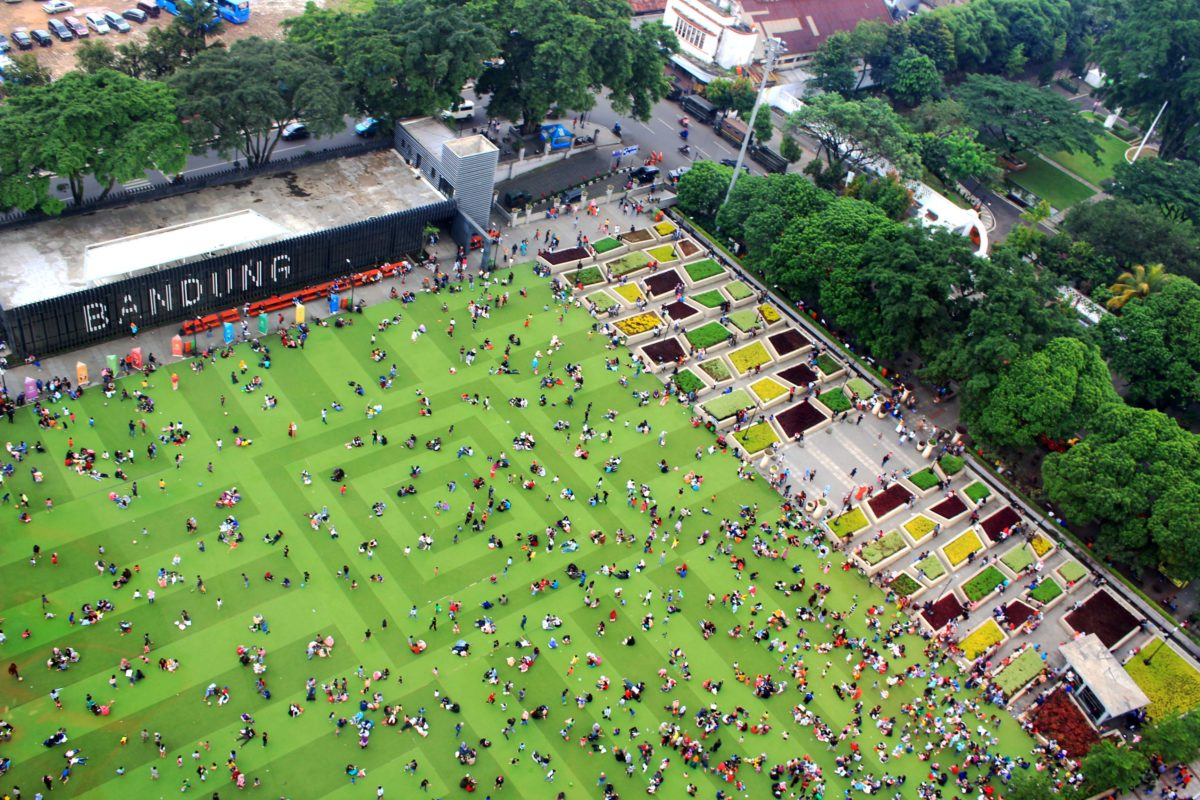
\includegraphics[width=0.5\textwidth]{ruang terbuka hijau.jpg}
	\caption{Contoh Ruang Terbuka Hijau}
\end{figure}

Pemanfaatan citra satelit merupakan salah satu cara agar dapat mengetahui luas RTH pada suatu kota. Citra Satelit adalah gambaran dari permukaan bumi yang didapatkan lansung dari satelit. Oleh karena itu, citra satelit dapat digunakan dalam pengidentifikasi RTH yang mana terdapatnya banyak pepohonan pada suatu wilayah. Perhitungan juga dapat dilakukan pada citra satelit ,dan hasil dari perhitungan luas RTH pada suatu wilayah diharapkan dapat memberikan dorongan untuk peningkatan dalam penghijauan agar dapat digunakan oleh pemerintah dalam merancang dan meningkatkan penghijauan di berbagai wilayah di Indonesia.
%insert image

Penelitian yang telah dilakukan Dr.~Veronica~Sri~Moertini, Fritz ~H.~Hutapea~SKom, dan Juan~A.~Kusjadi
%insert reference
menghasilkan data area hijau dari citra satelit pada Kota Bandung yang dibagi menjadi beberapa kelurahan atau kecamatan Kota Bandung. Hasil dari penelitian terdiri dari area hijau untuk 149 kelurahan di 30 kecamatan kota Bandung dan telah selesai dilakukan perhitungan.
%insert image

Pada Skripsi ini, akan dibangun sebuah laman web yang bertujuan untuk pemvisualisasian dari hasil penelitian area hijau Kota Bandung. Laman web yang akan dibangun harusnya dapat diakses melalui komputer atau laptop,handphone bersistem android ataupun iOS. Dan dalam pembuatanya akan dibantu dengan menggunakan \emph{Framework} Laravel, sehingga memudahkan pengembang untuk membangun laman web. Dengan adanya laman web pemvisualisasian ini juga akan memudahkan pengguna untuk mengetahui area-area hijau yang ada pada Kota Bandung.

\section{Rumusan Masalah}
Berdasarkan deskripsi dan latar belakang yang sudah dibahas bahwa rumusan masalah yang muncul adalah sebagai berikut:

\begin{enumerate}
	\item Bagaimana membuat sebuah laman web interaktif yang dapat membandingkan data dua buah kelurahan atau kecamatan Kota Bandung?
	\item Bagaimana cara pengguna untuk membandingkan atribut-atribut Citra Satelit dari kelurahan atau kecamatan Kota Bandung?
	\item Bagaiaman cara mengekstraksi data citra satelit pada HDFS ke \textit{local directory}?	
\end{enumerate}

\section{Tujuan}
Tujuan dari skripsi ini adalah:
\begin{enumerate}
	\item Membuat sebuah laman web interaktif yang dapat membandingkan dua buah kelurahan.
	\item Pengguna dapat memilih kelurahan atau kecamatan untuk sisi kiri dan kanan, untuk membandingkan atributnya.
	\item Data citra satelit yang didapatkan akan digunakan untuk memenuhi kebutuhan pada lawan web yang akan dibangun.
\end{enumerate}

\section{Detail Perkembangan Pengerjaan Skripsi}
Detail bagian pekerjaan skripsi sesuai dengan rencana kerja/laporan perkembangan terkahir :
	\begin{enumerate}
		\item \textbf {Melakukan survei kepada Fritz H. Hutapea SKom dan Juan A. Kusjadi terkait penenilitiannya}\\
		{\bf Status :} Ada sejak rencana kerja skripsi.\\
		{\bf Hasil :} Survei sudah dilakukan sekali dengan Fritz~H.~Hutapea~Skom pada tanggal 12 Desember 2022. Melakukan wawancara melalui sosial media \textit{Instagram}, Hasil wawancara mengenai file peta kelurahan bandung geoJSON. Survei kedua dilakukan sekali dengan Juan~A.~Kusjadi pada tanggal 30 Januari 2023. Wawancara yang dilakukan melalui \textit{Google Meet}, Hasil wawancara yang dilakukan berbincang mengenai data citra satelit. Data citra satelit yang didapatkan dari penyimpanan hadoop pada lab UNPAR(Universitas Katholik Parahyangan) dan mendaptkan dokumentasi skripsi Juan~A.~Kusjadi yang digunakan sebagai referensi utama dalam pengembangan laman web.
		
		\item \textbf{ Melakukan pengumpulan data hasil penelitian}\\
		{\bf Status :} Ada sejak rencana kerja skripsi.\\
		{\bf Hasil :} Pengumpulan data yang dilakukan dengan cara mendaftarkan diri untuk mendapatkan akun untuk dapat mengakses penyimpanan \textit{hadoop} lab UNPAR. Data hasil penelitian masih berupa format file ".txt" dan ".csv". Dari data hasil penilitian tersebut diunduh ke laptop pribadi melalui jaringan FTIS UNPAR. Data yang berupa format file ".txt" dapat diekstraksi menjadi sebuah gambar dari kelurahan atau kecamata Kota Bandung. Pengekstraksian data gambar dilakukan dengan menggunakan \textit{script python}. Dalam penggunaan \textit{script} terdapat beberapa \textit{library} dari bahasa pemrograman \textit{python} yaitu base64 digunakan untuk men-\textit{decode} data file menjadi format ".png" yang menghasilkan gambar berupa kumpulan \textit{tile} pembentuk gambar utuh dari kelurahan atau kecamatan dan \textit{Python PIL(Pillow)} sebagai penggabungan gambar dari kumpulan \textit{tile} menjadi sebuah gambar utuh dari kelurahan atau kecamatan.
		
		\item \textbf{Melakukan studi literatur dan studi eksplorasi mengenai \textit{framework} Apache Hadoop}\\
		{\bf Status :} Ada sejak rencana kerja skripsi.\\
		{\bf Hasil :} Pembelajaran mengenai studi literatur dan studi eksplorasi menghasilkan mengetahui \textit{Hadoop command-line} yang digunakan dalam pengunduhan data dari lab UNPAR.
		
		\item \textbf{Mempelajari ekstraksi data citra satelit yang disimpan pada HDFS}\\
		{\bf Status :} Ada sejak rencana kerja skripsi.\\
		{\bf Hasil :} Ekstrasi data citra satelit dapat menggunakan \textit{Hadoop command-line} seperti "\textit{get}" untuk pengambilan file data yang disimpan, dan \textit{command-line} seperti "\textit{scp}" untuk mengunduh file data yang tersimpan pada HDFS ke penyimpanan lokal laptop. Data file berupa ".txt" pada proses pengekstraksi data citra satelit menggunakan \textit{script} dengan bahasa \textit{Pyton}, dihasilkan gambar berupa banyak \textit{tile} dan banyak \textit{tile} digabungkan menjadi sebuah gambar dari kelurahan atau kecamatan dengan bantuan \textit{library PIL(Pyhton Pillow)} dari bahasa \textit{python}.

		\item \textbf{Mempelajari bahasa pemrograman php, html, css dan cara menggunakan framework laravel.}\\
		{\bf Status :} Ada sejak rencana kerja skripsi.\\
		{\bf Hasil :} Pembelajaran bahasa pemrograman php,html,css dan cara penggunaan framework laravel telah dilakukan, walaupun dalam pengembangan laman web masih belum dilakukan.

		\item \textbf{ Mempelajari kebutuhan laman web}\\
		{\bf Status :} Ada sejak rencana kerja skripsi \\
		{\bf Hasil :} Belum dikerjakan

		\item \textbf{Melakukan analisis kebutuhan laman web} \\
		{\bf Status :} Ada sejak rencana kerja skripsi.\\
		{\bf Hasil :} Analisis dari kebutuhan laman web berupa fitur-fitur yang akan tersedia pada laman web. Fitur-fitur yang akan tersedia pada laman web antara lain \textit{user} dapat memilih kelurahan atau kecamatan yang ingin dilihat. Setiap kecamtan atau kelurahan yang dipilih \textit{user} dapat melihat luas wilayah, luas area hijau, kebutuhan area hijau, gambar citra satelit/gambar luas area hijau, dan juga dapat mengakses ke halaman \textit{Google Maps} yang merujuk ke lokasi kelurahan atau kecamatan yang dipilih.

		\item \textbf{ Melakukan perancangan antar muka laman web}\\
		{\bf Status :} Ada sejak rencana kerja skripsi \\
		{\bf Hasil :} Belum dikerjakan

		\item \textbf{Membangun laman web bedasarkan framework Laravel}\\
		{\bf Status :} Ada sejak rencana kerja skripsi \\
		{\bf Hasil :} Belum dikerjakan
		
		\item \textbf{Melakukan pengujian pada laman web}\\
		{\bf Status :} Ada sejak rencana kerja skripsi \\
		{\bf Hasil :} Belum dikerjakan
		
		\item \textbf{Menulis dokumen skripsi}\\
		{\bf Status :} Ada sejak rencana kerja skripsi.\\
		{\bf Hasil :} Hasil dari penulisan dokumen skripsi terdiri dari Bab 1 dan Bab 2. Dokumentasi skripsi bab 1 berisikan latar belakang, rumusan masalah, tujuan, batasan masalah, metodologi, dan sistematika pembahasan dari pemvisualisasi hasil penelitian area hijau kelurahan atau kecamatan. Sedangkan dokumentasi skripsi pada bab 2 berisikan penjelasan teori-teori yang akan digunakan dalam membangun perangkat lunak. Penjelasan teori-teori yang digunakan antara lain yaitu \textit{Command-line interface} pada terminal, \textit{Haddop Distributed File System}, \textit{Python} dengan \textit{library PIL(Pillow)}, \textit{base64}, dan \textit{Framework laravel}. Untuk bab 3 belum diselesaikan sepenuhnya baru terdapat analisis dari perangkat lunak yang akan dikembangkan.

		\item \textbf{Melakukan studi literatur dan studi eksplorasi mengenai \textit{Base64}}\\
		{\bf Status :} Baru ditambahkan pada semester ini.\\
		{\bf Hasil :} Mempelajari algoritma Base64 yang digunakan untuk mengubah tipe data \textit{bytes} menjadi tipe data yang dapat dilihat(dan sebaliknya). Pada penggunaan base64 telah terdapat pada \textit{library} dari bahasa pemrograman \textit{python} yang tinggal digunakan. Dalam penggunaan base64 pada \textit{script} pengekstraksian gambar dilakukan dengan men-\textit{decode} text menjadi format file ".png".
	\end{enumerate}
\newpage

\section{Pencapaian Rencana Kerja}
Langkah-langkah kerja yang berhasil diselesaikan dalam Skripsi 1 ini adalah sebagai berikut:
\begin{enumerate}
\item Melakukan survei kepada Fritz H. Hutapea SKom dan Juan A. Kusjadi terkait penenilitiannya
\item Melakukan pengumpulan data hasil penelitian
\item Melakukan studi literatur dan studi eksplorasi mengenai framework Apache Hadoop
\item Mempelajari ekstraksi data citra satelit yang disimpan pada HDFS
\item Melakukan studi literatur dan studi eksplorasi mengenai \textit{Base64}
\item Melakukan analisis kebutuhan laman web.
\item Menulis dokumen skripsi
\end{enumerate}



\vspace{1cm}
\centering Bandung, \tanggal\\
%\vspace{2cm} 
\begin{figure}[h]
	\centering
	
\includegraphics[width=0.2\textwidth]{tandatangan.jpg}
\end{figure}
\nama \\ 
\vspace{1cm}

Menyetujui, \\
\ifdefstring{\jumpemb}{2}{
\vspace{1.5cm}
\begin{centering} Menyetujui,\\ \end{centering} \vspace{0.75cm}
\begin{minipage}[b]{0.45\linewidth}
% \centering Bandung, \makebox[0.5cm]{\hrulefill}/\makebox[0.5cm]{\hrulefill}/2013 \\
\vspace{2cm} Nama: \pembA \\ Pembimbing Utama
\end{minipage} \hspace{0.5cm}
\begin{minipage}[b]{0.45\linewidth}
% \centering Bandung, \makebox[0.5cm]{\hrulefill}/\makebox[0.5cm]{\hrulefill}/2013\\
\vspace{2cm} \pembB \\ Pembimbing Pendamping
\end{minipage}
\vspace{0.5cm}
}{
% \centering Bandung, \makebox[0.5cm]{\hrulefill}/\makebox[0.5cm]{\hrulefill}/2013\\
\vspace{2cm} \pembA \\ Pembimbing Tunggal
}
\end{document}

